\documentclass[11pt,a4paper]{article}

\usepackage[T1]{fontenc}
\usepackage[utf8]{inputenc}
\usepackage{lmodern}
\usepackage{microtype}
\usepackage[a4paper,margin=20mm]{geometry}
\usepackage{amsmath,amssymb,amsthm,mathtools,bm}
\usepackage{booktabs,longtable,tabularx,array,multirow}
\usepackage{enumitem}
\usepackage{xcolor}
\usepackage{hyperref}
\usepackage{setspace}
\usepackage{fancyhdr}
\usepackage{graphicx}
\usepackage{caption}
\usepackage{float}
\usepackage{listings}
\usepackage{tikz}
\usetikzlibrary{arrows.meta,calc,positioning,shapes.geometric,fit}

\definecolor{navy}{HTML}{17365D}
\definecolor{slate}{HTML}{394B59}
\definecolor{lightblue}{HTML}{EAF1F8}
\definecolor{lightgray}{HTML}{F3F5F7}
\definecolor{lightgreen}{HTML}{EAF6EE}
\definecolor{lightred}{HTML}{FBECEC}
\definecolor{amber}{HTML}{FFF3D6}
\definecolor{deepgreen}{HTML}{1E6B3A}
\definecolor{deepred}{HTML}{9B1C1C}
\definecolor{deepamber}{HTML}{8A5B00}
\definecolor{purple}{HTML}{5B3F8C}

\hypersetup{
  colorlinks=true,
  linkcolor=navy,
  citecolor=navy,
  urlcolor=navy,
  pdftitle={Microscopic QCD Scale Locking and the First Controlled Chronometric Shear},
  pdfsubject={All-orders scale-invariant QCD, threshold matching, clock drift, and equivalence-principle predictions}
}

\setstretch{1.045}
\setlength{\parindent}{0pt}
\setlength{\parskip}{0.50em}
\setlist[itemize]{leftmargin=1.55em,itemsep=0.16em,topsep=0.20em}
\setlist[enumerate]{leftmargin=1.75em,itemsep=0.16em,topsep=0.20em}
\captionsetup{font=small,labelfont=bf}

\pagestyle{fancy}
\fancyhf{}
\fancyhead[L]{\small\color{slate}QCD Chronometric Lock}
\fancyhead[R]{\small\color{slate}Technical note v0.5}
\fancyfoot[C]{\thepage}
\renewcommand{\headrulewidth}{0.3pt}

\newtheorem{definition}{Definition}[section]
\newtheorem{theorem}[definition]{Theorem}
\newtheorem{proposition}[definition]{Proposition}
\newtheorem{corollary}[definition]{Corollary}
\newtheorem{remark}[definition]{Remark}
\newtheorem{failure}[definition]{Failure mode}
\newtheorem{criterion}[definition]{Acceptance criterion}

\newcommand{\dd}{\mathrm{d}}
\newcommand{\Lag}{\mathcal{L}}
\newcommand{\M}{\mathcal{M}}
\newcommand{\MP}{M_{\mathrm P}}
\newcommand{\QCD}{\mathrm{QCD}}
\newcommand{\UV}{\mathrm{UV}}
\newcommand{\IR}{\mathrm{IR}}
\newcommand{\Tr}{\mathrm{Tr}}
\newcommand{\Pass}{\textcolor{deepgreen}{\textbf{PASS}}}
\newcommand{\Fail}{\textcolor{deepred}{\textbf{FAIL}}}
\newcommand{\Partial}{\textcolor{deepamber}{\textbf{PARTIAL}}}
\newcommand{\Open}{\textcolor{purple}{\textbf{OPEN}}}
\newcommand{\Conditional}{\textcolor{navy}{\textbf{COND.}}}
\newcolumntype{L}[1]{>{\raggedright\arraybackslash}p{#1}}
\newcolumntype{Y}{>{\raggedright\arraybackslash}X}

\newcommand{\statusbox}[2]{%
\begin{center}
\fcolorbox{#1}{#1!7}{\parbox{0.92\textwidth}{#2}}
\end{center}}

\begin{document}
\pagenumbering{gobble}

\begin{titlepage}
\thispagestyle{empty}
\vspace*{7mm}

{\color{navy}\rule{\textwidth}{1.2pt}}
\vspace{7mm}

{\fontsize{21}{25}\selectfont\bfseries\color{navy} Microscopic QCD Scale Locking and\\ the First Controlled Chronometric Shear\par}
\vspace{3mm}
{\Large An all-orders construction, exact threshold recursion, and a clock--equivalence-principle consistency relation\par}

\vspace{9mm}

\begin{center}
\begin{minipage}{0.93\textwidth}
\colorbox{lightblue}{\parbox{0.96\textwidth}{
\textbf{Main conclusion.} The local-RG argument of v0.4 can be replaced by an explicit all-orders Wilsonian construction in which the subtraction scale is the dynamical field $\chi$. Exact dilatation Ward identities then make every QCD transmutation scale homogeneous of degree one in $\chi$, so $\Lambda_{n_f}/\chi$ is constant whenever every coloured threshold is itself locked to $\chi$. Heavy-particle decoupling obeys an exact renormalization-group-invariant recursion. A single deliberately misaligned, vectorlike colour triplet produces the first controlled nonzero defect. At one loop,
\[
\dd\ln\frac{\Lambda_3}{\chi}
=\frac{2}{27}\,\varepsilon_\Psi\,\dd\theta+
O(\alpha_s\varepsilon_\Psi,\varepsilon_\Psi^2,\partial^2/\chi^2).
\]
This defect predicts a rank-one pattern across clock ratios and, for one long-range scalar and one QCD-dominated spurion, a parameter-free relation between anomalous clock redshift and differential free fall. The construction is an all-orders scale-invariant effective field theory, not yet a finite-parameter perturbatively renormalizable ultraviolet completion. The long-range version also has a serious radiative-naturalness problem that is isolated explicitly rather than concealed.
}}
\end{minipage}
\end{center}

\vfill

\begin{tabularx}{\textwidth}{@{}p{0.22\textwidth}X@{}}
Document status: & Technical research note; not peer reviewed \\
Version: & 0.5 \\
Date: & 16 August 2026 \\
Core construction: & Scale-invariant QCD with a dynamical subtraction scale, exact RGI threshold matching, one vectorlike coloured threshold, and a ratio-mode spurion \\
Accompanying files: & Symbolic/numerical verification script, machine-readable results, claim matrix, Markdown notes, and source package \\
Central limitation: & Exact all-orders scale invariance requires a Wilsonian tower of higher-dimensional operators; a finite microscopic UV completion and a technically natural ultralight ratio mode remain open
\end{tabularx}

\vspace{7mm}
{\color{navy}\rule{\textwidth}{1.2pt}}
\end{titlepage}

\pagenumbering{roman}

\begin{abstract}
We replace the previous local renormalization-group ansatz for $\Lambda_{\QCD}/\chi$ by an explicit $d=4-2\epsilon$ bare functional. The ordinary subtraction mass is promoted to $\mu_\chi=z\chi^{1/(1-\epsilon)}$, and all bare gauge, Yukawa and scalar couplings are defined with the corresponding powers of $\mu_\chi$. Renormalization generates the symmetry-required tower of scale-invariant higher-dimensional operators. The resulting construction is renormalized order by order as a Wilsonian effective field theory and has an exact dilatation Ward identity; a path-integral implementation provides a formal nonperturbative definition. In a vacuum with $f=\langle\chi\rangle\neq0$, every physical pole or gap is therefore of the form $M_n=f\,\mathcal F_n$ and, in the adiabatic local limit, $\Lambda_{n_f}(x)=c_{n_f}\chi(x)$ up to derivative corrections. This is stronger and more microscopic than choosing a matching scale proportional to $\chi$, but it is not a power-counting-renormalizable ultraviolet completion.

We then derive an exact all-orders threshold theorem. If a theory with $n$ active coloured fermions is matched to one with $n-1$, dimensional analysis of renormalization-group-invariant quantities gives $\Lambda_{n-1}=\widehat m_j\mathcal F_j(\Lambda_n/\widehat m_j)$. Defining $A_j=\partial\ln\mathcal F_j/\partial\ln(\Lambda_n/\widehat m_j)$, the QCD lock defect obeys
\[
\delta_{n-1}=A_j\delta_n+(1-A_j)\epsilon_j,
\qquad
\delta_n=\dd\ln(\Lambda_n/\chi),\quad
\epsilon_j=\dd\ln(\widehat m_j/\chi).
\]
This statement is exact; scheme and loop dependence reside only in the physical response $A_j$.

A conventional real scalar $S$ and one anomaly-free vectorlike Dirac fermion $\Psi\sim({\bf3},{\bf1},0)$ generate a controlled violation. The renormalizable mass $M_\Psi=y_\chi\chi+y_SS$ is exactly locked when $S/\chi$ is constant. Writing $S/\chi=r e^\theta$ gives $\dd\ln(M_\Psi/\chi)=\varepsilon_\Psi\dd\theta$, where $\varepsilon_\Psi=y_Sr/(y_\chi+y_Sr)$. For the $7\to6\to5\to4\to3$ threshold chain, with the top, bottom and charm thresholds locked, the leading coefficient telescopes to $2/27$. The physical ratio eigenvalue of the scalar alignment Hessian is positive. An exactly global-scale-invariant completion retains the expected flat radial dilaton direction; a locally Weyl-gauged or softly lifted completion with $m_\chi^2>0$ is positive definite. A 50,000-point scan of the lifted completion found no negative eigenvalue in the stated positive-coupling domain.

The low-energy defect produces
\[
\mathcal S_{AB}
=(\Delta K_\mu-\Delta K_q)\frac{2}{27}\varepsilon_\Psi\dd\theta+\cdots.
\]
Using the leading clock sensitivities $K_\mu({\rm Sr})=0$, $K_\mu({\rm CaF})=-1/2$ and $K_\mu({\rm Cs})=-1$ yields $\mathcal S_{\rm Sr/Cs}=2\mathcal S_{\rm Sr/CaF}$. If the same unscreened scalar mediates a long-range force, standard dilaton charges imply
\[
\frac{\beta_{AB}}{\eta_{CD}}
=-\frac{\Delta K_\mu-\Delta K_q}{\Delta Q'_{\widehat m}{}^{CD}}.
\]
For Ti/Pt this gives, in the leading gluonic approximation, $\beta_{\rm Sr/CaF}\simeq150.38\,\eta_{\rm Ti/Pt}$ and $\beta_{\rm Sr/Cs}\simeq300.76\,\eta_{\rm Ti/Pt}$, up to ratio and sign conventions. This is the first nonzero, dimensionless clock--equivalence-principle consistency prediction of the programme. Its assumptions and failure modes are stated explicitly.
\end{abstract}

\setcounter{tocdepth}{1}
\begingroup
\small
\setlength{\parskip}{0pt}
\tableofcontents
\endgroup
\clearpage
\pagenumbering{arabic}

\section{Executive verdict}

\begin{table}[H]
\centering
\caption{Status of the decisive QCD step.}
\begin{tabularx}{\textwidth}{@{}L{0.30\textwidth}L{0.12\textwidth}Y@{}}
\toprule
Requirement & Status & Result \\
\midrule
Explicit all-orders QCD lock & \Pass & A dynamical-subtraction-scale bare functional and exact dilatation Ward identity make $\Lambda_n/\chi$ constant when all thresholds are locked. \\
Finite-parameter perturbative UV completion & \Open & Exact scale-invariant regularization generates an infinite tower of higher-dimensional interactions. \\
Formal nonperturbative definition & \Conditional & A scale-invariant path-integral measure exists, but constructive positivity and a complete nonperturbative QCD-plus-$\chi$ solution are not proved here. \\
All-orders threshold propagation & \Pass & The RGI recursion $\delta_{n-1}=A_j\delta_n+(1-A_j)\epsilon_j$ is exact. \\
Renormalizable controlled-breaking sector & \Pass & $S$ and vectorlike $\Psi$ have conventional two-derivative kinetics and dimension-four interactions; the full finite counterterm basis is understood. \\
Lorentzian unitarity & \Pass & The added sector is an ordinary vectorlike gauge theory with positive kinetic terms and no gauge anomaly. \\
Positive physical spectral density & \Pass & Gauge-invariant operators of the conventional sector admit the standard positive Hilbert-space interpretation; no fourth-order elementary field is used. \\
Stable condensate/alignment & \Conditional & The ratio mode is positive for $\lambda_S>0$. Exact global scale symmetry leaves one flat radial dilaton; a gauged or lifted completion with $m_\chi^2>0$ is positive definite, and 50,000 random lifted points passed. \\
Leading nonzero QCD defect & \Pass & One fundamental Dirac colour triplet gives $\mathcal D_{\Psi\to3}^{(1)}=2/27$. \\
Clock prediction & \Pass & At leading rank one, $\mathcal S_{\rm Sr/Cs}=2\mathcal S_{\rm Sr/CaF}$. \\
Clock--EP prediction & \Pass & Same-source elimination gives a coupling-independent $\beta_{AB}/\eta_{CD}$ relation. \\
Long-range observable realization & \Conditional & A light ratio mode is required; its mass is radiatively sensitive to the coloured threshold and needs additional protection. \\
Collider and relic safety & \Conditional & Trivial for a superheavy $\Psi$ with reheating below its mass; lower masses require a dedicated decay and collider model. \\
Absolute novelty priority & \Open & The ingredients are known; the restricted defect-recursion and clock--EP synthesis appears new but needs citation-chain and specialist review. \\
\bottomrule
\end{tabularx}
\end{table}

\statusbox{navy}{\textbf{Strongest defensible result.}
\[
\boxed{
\begin{gathered}
\text{exact scale Ward identity}
+\text{locked coloured thresholds}
\Longrightarrow \Lambda_{\QCD}/\chi=\mathrm{constant},\\[1mm]
\text{one threshold misalignment}
\Longrightarrow
\mathcal S_{AB}\neq0,
\quad
\frac{\beta_{AB}}{\eta_{CD}}
=-\frac{\Delta K_\mu-\Delta K_q}{\Delta Q'_{\widehat m}{}^{CD}}.
\end{gathered}}
\]
The microscopic lock is exact inside an all-orders scale-invariant Wilsonian QFT. The first violation is calculable, rank one, and experimentally cross-checkable.}

\section{The target: an exact QCD lock, not a choice of renormalization scale}

The v0.4 construction wrote the QCD scale schematically as
\[
\Lambda_{\QCD}=\chi\,
\exp\left[-\int^{g_s(\chi)}\frac{\dd g}{\beta_s(g)}\right],
\]
and imposed boundary data at a matching scale proportional to $\chi$. That is a valid local-RG parametrization, but by itself it does not answer the microscopic question: why is the subtraction standard that defines the quantum theory co-moving with $\chi$, and why do counterterms preserve that statement to every order?

The upgraded target has four parts.

\begin{enumerate}
  \item The bare functional must contain no independent dimensionful subtraction parameter.
  \item Renormalization must preserve an exact dilatation Ward identity in the enlarged theory.
  \item Every coloured threshold must have an RGI mass proportional to $\chi$ in the exact-lock limit.
  \item The first departure from this trajectory must be represented by an explicit renormalizable spurion whose propagation to low-energy QCD is calculable.
\end{enumerate}

The solution below uses the scale-invariant regularization programme of Refs.~\cite{Tamarit2013,Ghilencea2016,HerreroValea2020}. Its cost is important: the exact quantum theory is a Wilsonian EFT with infinitely many symmetry-related operators. Thus ``all orders'' here means an explicit all-orders renormalized functional, not a proof of a finite-parameter ultraviolet completion.

\section{All-orders microscopic scale-invariant QCD}
\label{sec:allorders}

\subsection{Field content and dimensions}

Let $\chi$ be the positive radial order parameter generated by the safe hidden sector of v0.4. Along the Higgs portal valley,
\[
h=\zeta_h\chi,
\]
so every Standard Model quark mass is
\[
m_q=y_q\frac{h}{\sqrt2}
=\widehat y_q\chi,
\qquad
\widehat y_q\equiv\frac{y_q\zeta_h}{\sqrt2}.
\]
The QCD sector also contains, temporarily, a vectorlike coloured fermion $\Psi$ that will be used to create a controlled threshold defect. In the exact-lock limit its RGI mass is proportional to $\chi$.

Work in
\[
d=4-2\epsilon.
\]
A scalar has engineering dimension $1-\epsilon$. Therefore
\[
\boxed{
\mu_\chi(x)=z\,\chi(x)^{1/(1-\epsilon)}
}
\label{eq:muchi}
\]
has mass dimension one. Here $z$ is dimensionless and plays the role ordinarily assigned to the dimensionless ratio $\mu/f$ after spontaneous symmetry breaking.

\subsection{Bare functional}

A representative bare QCD-plus-scale-sector functional is
\begin{align}
S_0^{(d)}=\int\dd^dx\sqrt{-g}\Bigg[&
-\frac14 Z_G G^a_{\mu\nu}G^{a\mu\nu}
+\sum_q Z_q\bar q i\gamma^\mu D_\mu q
+Z_\Psi\bar\Psi i\gamma^\mu D_\mu\Psi
\nonumber\\
&+\frac12Z_\chi(\partial\chi)^2
+\frac12Z_S(\partial S)^2
-V_0(\chi,S,H)
\nonumber\\
&-\sum_q \mu_\chi^\epsilon Z_{y_q}y_q\,\bar qHq
-\bar\Psi\bigl(Z_{y_\chi}y_\chi\chi+Z_{y_S}y_SS\bigr)\Psi
\nonumber\\
&+\sum_{k\ge1}\frac{c_{0,k}}{\chi^{2k/(1-\epsilon)}}
\mathcal O_{d+2k}
\Bigg].
\label{eq:bareaction}
\end{align}
The gauge coupling appearing in $D_\mu$ is
\[
g_{s,0}=\mu_\chi^\epsilon Z_g g_s,
\]
and dimensionless scalar quartics carry $\mu_\chi^{2\epsilon}$. The last line represents the complete tower of scale-invariant local operators required by renormalization. The notation is schematic because operator mixing must be resolved in any fixed loop calculation; the key point is that every coefficient is dimensionless and every apparent inverse mass is a power of the field $\chi$.

Expanding about the broken vacuum,
\[
\chi=f+\sigma,
\]
turns Eq.~\eqref{eq:muchi} into a non-polynomial series in $\sigma/f$. Poles in $\epsilon$ multiply this series and generate finite higher-dimensional vertices. The ordinary renormalizable QCD action is recovered when fluctuations $\sigma/f$ are negligible, but the exact scale-invariant completion necessarily retains the full tower. This is why exact scale symmetry and ordinary running can coexist, and also why the completion is not power-counting renormalizable \cite{Tamarit2013,Ghilencea2016,HerreroValea2020}.

\subsection{Exact Ward identity}

Let $\Gamma$ be the renormalized one-particle-irreducible effective action including the complete symmetry-required basis. In flat spacetime its exact global scale Ward operator is schematically
\[
\mathcal D\Gamma
\equiv
\left[
\int\dd^dx\sum_i\Delta_i\Phi_i(x)
\frac{\delta}{\delta\Phi_i(x)}
-f\frac{\partial}{\partial f}
\right]\Gamma=0,
\label{eq:ward}
\]
where $\Phi_i$ denotes every renormalized field and $\Delta_i$ its scaling dimension, including anomalous contributions in a chosen renormalized basis. The path-integral construction of Ref.~\cite{HerreroValea2020} implements the same statement through a modified functional measure and is intended to extend beyond perturbation theory.

The identity does not force the beta functions to vanish. Running is with respect to the dimensionless parameter $z$, and in the broken phase it reproduces ordinary RG evolution. What vanishes is the anomaly of the \emph{enlarged} theory: the scale transformed by the RG is itself a dynamical field.

\begin{theorem}[Homogeneity of physical gaps]
Assume Eq.~\eqref{eq:ward}, a stable vacuum $f=\langle\chi\rangle>0$, and no second independent dimensionful order parameter. Every physical pole mass, inverse correlation length or spectral gap satisfies
\[
\boxed{
M_A(f)=f\,\mathcal F_A(g_i(z),y_i(z),\lambda_i(z),\ldots).
}
\label{eq:homogeneity}
\]
Consequently, under a common adiabatic rescaling of the scale field, $M_A/\chi$ is invariant.
\end{theorem}

\begin{proof}
The pole condition is a dimension-one observable. Exact scale invariance maps a vacuum with order parameter $f$ to a vacuum with order parameter $\lambda f$, while leaving dimensionless renormalized data unchanged. Therefore $M_A(\lambda f)=\lambda M_A(f)$. Euler homogeneity gives Eq.~\eqref{eq:homogeneity}. The argument applies to a nonperturbative mass gap if the scale-invariant path integral exists and the relevant gauge-invariant correlator has an isolated positive spectral scale.
\end{proof}

For QCD with $n_f$ active flavours,
\[
\boxed{
\Lambda_{n_f}(x)=c_{n_f}\chi(x)
}
\label{eq:exactlock}
\]
in the adiabatic, exact-lock limit. The constant $c_{n_f}$ is exponentially sensitive to dimensionless boundary data, just as ordinary $\Lambda_{\QCD}$ is, but it is dimensionless.

\subsection{Local derivative expansion}

A varying $\chi(x)$ is not identical to a sequence of constant vacua. The local mass gap therefore has a covariant derivative expansion,
\begin{align}
\Lambda_{n_f}(x)=c_{n_f}\chi(x)\Bigg[1
&+c_{\Box}\frac{\Box\chi}{\chi^3}
+c_{\partial}\frac{(\nabla\chi)^2}{\chi^4}
\nonumber\\
&+O\!\left(\frac{\nabla^4}{\chi^4},
\frac{\mathcal R}{\chi^2}\right)\Bigg].
\label{eq:derivative}
\end{align}
Thus the exact algebraic lock is the zeroth-order term in a controlled adiabatic expansion. In terrestrial clock and fifth-force applications the relevant scalar variation length is macroscopic, whereas $\Lambda_{\QCD}^{-1}$ is femtoscopic, so the derivative corrections are normally negligible. They become important in early-universe phase transitions, defects and rapidly varying backgrounds.

\begin{remark}[What has and has not been solved]
Equations~\eqref{eq:bareaction}--\eqref{eq:exactlock} replace the phrase ``choose $\mu\propto\chi$'' by a microscopic all-orders rule for the bare quantum functional. They do not provide an asymptotically safe or finite-parameter UV completion. The theory is predictive below a cutoff only after a power counting and boundary conditions for its Wilson coefficients are specified.
\end{remark}

\section{An exact all-orders threshold recursion}
\label{sec:threshold}

The all-orders lock is useful only if it survives the removal of heavy coloured states. Threshold matching is therefore the decisive step.

\subsection{RG-invariant variables}

For a theory with $n$ active coloured fermions, define an RGI strong scale and an RGI heavy mass by
\begin{align}
\Lambda_n
&=\mu\,
\exp\left[-\int^{g_n(\mu)}\frac{\dd g}{\beta_n(g)}\right]
\times \mathcal C_n,
\label{eq:rgilambda}\\
\widehat m_j
&=m_j(\mu)
\exp\left[-\int^{g_n(\mu)}\frac{\gamma_{m,j}(g)}{\beta_n(g)}\dd g\right]
\times \mathcal C_{m,j},
\label{eq:rgimass}
\end{align}
where the constants $\mathcal C$ fix conventions. Matching the $n$-flavour theory to the $(n-1)$-flavour theory at a heavy threshold can depend only on the two physical dimension-one quantities $\Lambda_n$ and $\widehat m_j$.

\begin{theorem}[Exact threshold map]
For one isolated heavy threshold,
\[
\boxed{
\Lambda_{n-1}
=\widehat m_j\,
\mathcal F_j\!\left(\frac{\Lambda_n}{\widehat m_j}\right),
}
\label{eq:thresholdmap}
\]
where $\mathcal F_j$ is a dimensionless, scheme-independent map once the RGI conventions are fixed. Define
\[
A_j\equiv
\frac{\partial\ln\mathcal F_j(x)}{\partial\ln x},
\qquad x=\frac{\Lambda_n}{\widehat m_j}.
\label{eq:Aj}
\]
Then
\[
\boxed{
\dd\ln\Lambda_{n-1}
=A_j\dd\ln\Lambda_n
+(1-A_j)\dd\ln\widehat m_j.
}
\label{eq:thresholdresponse}
\]
\end{theorem}

\begin{proof}
Equation~\eqref{eq:thresholdmap} follows from dimensional analysis of physical RGI quantities and decoupling. Taking a logarithmic differential gives
\[
\dd\ln\Lambda_{n-1}
=\dd\ln\widehat m_j
+A_j(\dd\ln\Lambda_n-\dd\ln\widehat m_j),
\]
which is Eq.~\eqref{eq:thresholdresponse}. Higher-loop matching changes $\mathcal F_j$ and therefore $A_j$, but cannot alter the form of the relation. All-order low-energy theorems express the response to the heavy mass through derivatives of the QCD decoupling constants \cite{Chetyrkin1998}.
\end{proof}

Define the lock defects
\[
\delta_n\equiv\dd\ln\frac{\Lambda_n}{\chi},
\qquad
\epsilon_j\equiv\dd\ln\frac{\widehat m_j}{\chi}.
\label{eq:defects}
\]
Subtracting $\dd\ln\chi$ from Eq.~\eqref{eq:thresholdresponse} gives the exact recursion
\[
\boxed{
\delta_{n-1}=A_j\delta_n+(1-A_j)\epsilon_j.
}
\label{eq:defectrecursion}
\]

Several immediate consequences matter.

\begin{itemize}
  \item If $\delta_n=0$ and $\epsilon_j=0$, then $\delta_{n-1}=0$. Exact locking survives decoupling to all orders.
  \item A threshold mismatch enters with weight $1-A_j$ and is subsequently diluted or transmitted by all lower threshold responses.
  \item No renormalization-scheme-dependent coupling or arbitrary matching scale appears in Eq.~\eqref{eq:defectrecursion}; those details are packaged in the physical response $A_j$.
\end{itemize}

For a chain of thresholds $N\to N-1\to\cdots\to3$, let $A_n$ denote the response at the $n\to n-1$ step. Iteration gives
\[
\boxed{
\delta_3
=\left(\prod_{n=4}^{N}A_n\right)\delta_N
+\sum_{n=4}^{N}
(1-A_n)
\left(\prod_{k=4}^{n-1}A_k\right)
\epsilon_n,
}
\label{eq:multithreshold}
\]
where the empty product equals one. Equation~\eqref{eq:multithreshold} is the all-orders transport law for chronometric QCD defects.

\subsection{One-loop limit}

At one loop for $SU(3)$ with $n$ active Dirac fundamentals,
\[
b_n=11-\frac{2n}{3},
\]
and continuity at the heavy threshold gives
\[
\Lambda_{n-1}^{b_{n-1}}
=\widehat m_j^{b_{n-1}-b_n}\Lambda_n^{b_n}.
\]
Therefore
\[
A_j^{(1)}=\frac{b_n}{b_{n-1}},
\qquad
1-A_j^{(1)}=\frac{b_{n-1}-b_n}{b_{n-1}}.
\label{eq:oneA}
\]
For a Dirac fermion in a general colour representation $R$,
\[
b_{n-1}-b_n=\frac43T(R).
\]
After all lower Standard Model heavy-quark thresholds have been traversed, the leading response of the three-flavour scale to one isolated extra threshold is
\[
\boxed{
\mathcal D_{R\to3}^{(1)}=\frac{4T(R)}{27}.
}
\label{eq:generalrep}
\]
For the fundamental representation, $T({\bf3})=1/2$, hence
\[
\boxed{
\mathcal D_{{\bf3}\to3}^{(1)}=\frac{2}{27}.
}
\label{eq:two27}
\]
The coefficient $2/27$ is familiar from heavy-quark and dilaton low-energy theorems. The new role assigned to it here is as the leading transmission coefficient from a microscopic threshold lock defect to chronometric shear.

\section{A renormalizable controlled-breaking sector}
\label{sec:breaking}

\subsection{Fields and action}

Add one real scalar $S$ and one vectorlike Dirac fermion
\[
\Psi\sim({\bf3},{\bf1},0)
\]
under $SU(3)_c\times SU(2)_L\times U(1)_Y$. The minimal Lagrangian is
\begin{align}
\Lag_{\Psi S}={}&
\bar\Psi\left(i\!\not\!D-y_\chi\chi-y_SS\right)\Psi
-\frac12(\partial S)^2
-V_{\chi S},
\label{eq:psislag}\\
V_{\chi S}={}&
V_\chi(\chi)
+\frac{\lambda_S}{4}(S^2-r^2\chi^2)^2
+\Delta V_{\rm ct}(\chi,S).
\label{eq:alignpotential}
\end{align}
Here $V_\chi$ denotes the common-scale sector. In an exactly global-scale-invariant realization it has a flat radial direction after spontaneous breaking, as required for the dilaton Goldstone mode. In a locally Weyl-invariant completion that direction can be gauge, while controlled soft or dynamical breaking can instead supply a positive physical curvature $m_\chi^2$. The displayed perfect square defines a convenient renormalized alignment surface. Because $y_SS\bar\Psi\Psi$ breaks $S\to-S$, the full counterterm basis $\Delta V_{\rm ct}$ includes the allowed mixed quartics $S\chi^3$ and $S^3\chi$, with coefficients proportional to the same breaking spurion. The $S$--$\Psi$ matter sub-sector remains power-counting renormalizable; the point is not that the perfect square is radiatively exact, but that the vacuum ratio $r$ and its curvature are renormalized physical parameters.

The limit
\[
y_S\to0
\]
removes the threshold mismatch and separates $S$ from the coloured fermion. Every non-universal effect derived below is therefore proportional to a technically controlled spurion.

\subsection{Vacuum and scalar stability}

Ignoring the small spurion counterterms for the analytic benchmark, the aligned vacuum is
\[
\chi=f,
\qquad
S=rf.
\]
The alignment contribution to the Hessian in the basis $(\chi,S)$ is
\[
H_{\rm align}
=2\lambda_Sf^2
\begin{pmatrix}
r^4&-r^3\\
-r^3&r^2
\end{pmatrix}.
\label{eq:alignHessian}
\]
It has eigenvalues
\[
0,
\qquad
2\lambda_Sf^2r^2(1+r^2).
\]
The zero mode is the common radial scaling direction. This must be interpreted according to the completion:
\begin{itemize}
  \item for exact spontaneously broken \emph{global} scale symmetry, $m_\chi^2=0$ and this is the physical massless dilaton required by Goldstone's theorem; the Hessian is positive semidefinite, not unstable;
  \item for a locally Weyl-invariant completion, the common radial direction may be gauge;
  \item for a softly or dynamically lifted completion, let $m_\chi^2>0$ denote the physical radial curvature.
\end{itemize}
In the lifted case,
\[
H_{\rm total}
=
\begin{pmatrix}
m_\chi^2+2\lambda_Sf^2r^4&-2\lambda_Sf^2r^3\\
-2\lambda_Sf^2r^3&2\lambda_Sf^2r^2
\end{pmatrix},
\]
with
\[
\Tr H_{\rm total}
=m_\chi^2+2\lambda_Sf^2r^2(1+r^2)>0,
\]
and
\[
\boxed{
\det H_{\rm total}
=2\lambda_Sf^2r^2m_\chi^2>0.
}
\label{eq:positiveHessian}
\]
Thus the ratio mode is locally stable for $\lambda_S>0$ and $r\neq0$. The global-scale version has one expected flat mode; the lifted version is strictly positive definite for $m_\chi^2>0$. The accompanying script verified the factorization symbolically and sampled 50,000 positive lifted parameter points without a negative scalar eigenvalue.

\subsection{The ratio mode and threshold defect}

Parametrize the relative alignment by
\[
\frac{S}{\chi}=r e^{\theta(x)}.
\label{eq:theta}
\]
The heavy mass is
\[
M_\Psi
=\chi\left(y_\chi+y_Sr e^\theta\right).
\]
At $\theta=0$,
\[
\boxed{
\dd\ln\frac{M_\Psi}{\chi}
=\varepsilon_\Psi\dd\theta,
\qquad
\varepsilon_\Psi
=\frac{y_Sr}{y_\chi+y_Sr}.
}
\label{eq:epsilonpsi}
\]
The parameter $\varepsilon_\Psi$ is bounded between zero and one for positive couplings and directly measures how much of the coloured mass is carried by the misaligning field rather than the universal scale field.

The added sector is conventional: two-derivative scalar and fermion kinetics, a vectorlike gauge representation, and a Hamiltonian bounded below in the stable domain. It therefore avoids the Lorentzian and spectral problems associated with fourth-order elementary scalars.

\section{The first nonzero QCD lock defect}
\label{sec:firstdefect}

Above the exotic threshold there are seven active Dirac colour fundamentals: the six Standard Model quarks and $\Psi$. Assume the scale-invariant microscopic theory gives
\[
\delta_7=0,
\]
and that the top, bottom and charm masses remain exactly locked,
\[
\epsilon_t=\epsilon_b=\epsilon_c=0.
\]
Only $\Psi$ carries the ratio-mode defect of Eq.~\eqref{eq:epsilonpsi}. The exact result is
\[
\boxed{
\dd\ln\frac{\Lambda_3}{\chi}
=\mathcal D_{\Psi\to3}\,
\varepsilon_\Psi\dd\theta,
\qquad
\mathcal D_{\Psi\to3}
=(1-A_\Psi)A_tA_bA_c.
}
\label{eq:exactD}
\]
The four $A$ coefficients are the all-orders physical responses defined in Eq.~\eqref{eq:Aj}. They can be calculated to any available perturbative order from QCD beta functions and decoupling constants; Eq.~\eqref{eq:exactD} remains true nonperturbatively whenever the RGI threshold map exists.

At one loop,
\[
A_\Psi=\frac{19}{21},
\qquad
A_t=\frac{21}{23},
\qquad
A_b=\frac{23}{25},
\qquad
A_c=\frac{25}{27}.
\]
The product telescopes:
\begin{align}
\mathcal D_{\Psi\to3}^{(1)}
&=\left(1-\frac{19}{21}\right)
\frac{21}{23}\frac{23}{25}\frac{25}{27}
\nonumber\\
&=\boxed{\frac{2}{27}}.
\label{eq:telescope}
\end{align}
Equivalently,
\[
\boxed{
\Lambda_3^9
=\Lambda_7^{19/3}
\left(M_\Psi m_tm_bm_c\right)^{2/3}
}
\label{eq:lambdaidentity}
\]
at leading order. Taking a differential and imposing exact lock on $\Lambda_7,t,b,c$ reproduces Eq.~\eqref{eq:telescope}.

The first controlled result is therefore
\[
\boxed{
\dd\ln\frac{\Lambda_3}{\chi}
=\frac{2}{27}\varepsilon_\Psi\dd\theta
+O\!\left(
\alpha_s\varepsilon_\Psi,
\varepsilon_\Psi^2,
\frac{\partial^2}{\chi^2}
\right).
}
\label{eq:qcddefect}
\]
The correction labelled $\alpha_s\varepsilon_\Psi$ is shorthand for the calculable higher-order threshold responses at $M_\Psi,m_t,m_b,m_c$, not an uncontrolled ambiguity. The derivative term is the local-adiabatic correction of Eq.~\eqref{eq:derivative}.

\begin{remark}[Why the coefficient is physically useful]
The bare number $2/27$ is not a new QCD theorem. Its utility here is structural: the first failure of universal scale locking is not arbitrary. It is filtered by decoupling and arrives at hadronic scales with a fixed leading coefficient. A different colour representation changes the coefficient to $4T(R)/27$; multiple independent misaligned thresholds raise the rank of the clock network.
\end{remark}

\section{From the QCD defect to chronometric shear}
\label{sec:clocks}

\subsection{Low-energy variables}

Write a low-energy clock ratio as a function of dimensionless constants,
\[
\frac{\nu_A}{\nu_B}
=\mathcal R_{AB}
\left(
\alpha,
\mu,
X_q,\ldots
\right),
\]
where
\[
\mu=\frac{m_p}{m_e},
\qquad
X_q=\frac{\widehat m}{\Lambda_3}.
\]
Its differential is
\[
\boxed{
\mathcal S_{AB}
\equiv\dd\ln\frac{\nu_A}{\nu_B}
=\Delta K_\alpha\dd\ln\alpha
+\Delta K_\mu\dd\ln\mu
+\Delta K_q\dd\ln X_q+\cdots.
}
\label{eq:sheargeneral}
\]
This is the chronometric-shear one-form of v0.3.

For the benchmark spurion, the electromagnetic coupling, the light-quark masses and the electron mass remain locked to $\chi$ at the matching scale. The leading gluonic deformation is therefore
\[
\dd\ln\alpha=0,
\qquad
\dd\ln\mu\simeq\delta_3,
\qquad
\dd\ln X_q=-\delta_3.
\label{eq:pureqcdvariation}
\]
The approximation in $\dd\ln\mu$ neglects the light-quark sigma-term fraction of the proton mass; retaining $K_q$ consistently captures the leading non-gluonic correction. Combining Eqs.~\eqref{eq:qcddefect}--\eqref{eq:pureqcdvariation} gives
\[
\boxed{
\mathcal S_{AB}
=(\Delta K_\mu-\Delta K_q)
\frac{2}{27}\varepsilon_\Psi\dd\theta
+\cdots.
}
\label{eq:shearprediction}
\]

\subsection{A rank-one clock pattern}

For the explicitly ordered ratios used here, current clock sensitivity tables give the leading electron--proton mass-ratio coefficients
\[
K_\mu({\rm Sr})=0,
\qquad
K_\mu({\rm CaF})=-\frac12,
\qquad
K_\mu({\rm Cs})=-1
\]
\cite{Elder2025}. Neglecting the subleading $K_q$ differences for the first benchmark,
\begin{align}
\boxed{
\mathcal S_{\rm Sr/CaF}
=\frac{1}{27}\varepsilon_\Psi\dd\theta+\cdots,
}
\label{eq:srcaf}\\
\boxed{
\mathcal S_{\rm Sr/Cs}
=\frac{2}{27}\varepsilon_\Psi\dd\theta+\cdots.
}
\label{eq:srcs}
\end{align}
Eliminating the unobservable local field excursion gives the first dimensionless consistency relation:
\[
\boxed{
\mathcal S_{\rm Sr/Cs}
=2\mathcal S_{\rm Sr/CaF}
}
\label{eq:rankone}
\]
at leading order.

This is a rank-one statement. Every clock ratio responds to the same one-form $\varepsilon_\Psi\dd\theta$, multiplied by a known sensitivity. A second independent threshold mismatch would generically break Eq.~\eqref{eq:rankone} and increase the rank of the clock-response matrix.

\begin{failure}[Nuclear and electromagnetic corrections]
Real clocks are not pure powers of $\mu$. Relativistic electronic structure, nuclear magnetic moments, light-quark masses and electromagnetic binding introduce $K_\alpha$ and $K_q$ corrections. Equation~\eqref{eq:rankone} is therefore the leading gluonic line, not an exact Standard Model identity. A precision analysis must use ab initio sensitivities and the higher-order $A_j$ responses.
\end{failure}

\section{A parameter-free clock--equivalence-principle relation}
\label{sec:EP}

\subsection{Scalar couplings}

Let the canonically normalized long-wavelength ratio mode be $a=f_a\theta$ and define dimensionless scalar couplings using $\varphi=a/\MP$. The QCD coupling generated by Eq.~\eqref{eq:qcddefect} is
\[
\boxed{
 d_g
\equiv
\frac{\partial}{\partial\varphi}
\ln\frac{\Lambda_3}{\chi}
=\frac{2}{27}\varepsilon_\Psi\frac{\MP}{f_a}+\cdots.
}
\label{eq:dg}
\]
In the pure threshold benchmark,
\[
d_{\widehat m}=0,
\qquad
d_e=0.
\]
The approximate scalar coupling of an atom $A$ is then, following the dilaton-charge decomposition of Damour and Donoghue \cite{DamourDonoghue2010},
\[
\alpha_A
\simeq d_g^*
+\left[(d_{\widehat m}-d_g)Q'_{\widehat m}+d_eQ'_e\right]_A.
\label{eq:atomcharge}
\]
Hence the composition-dependent difference is
\[
\boxed{
\alpha_C-\alpha_D
=-d_g\Delta Q'_{\widehat m}{}^{CD}.
}
\label{eq:chargedifference}
\]
If a source $X$ carries scalar charge $\alpha_X$ and the scalar range exceeds the source--experiment separation, the Eotvos parameter is
\[
\boxed{
\eta_{CD}
\simeq -d_g\alpha_X\Delta Q'_{\widehat m}{}^{CD}.
}
\label{eq:eta}
\]
The same source produces a differential anomalous clock redshift. With the convention
\[
\dd\ln\frac{\nu_A}{\nu_B}
=\beta_{AB}\,\dd U,
\]
one obtains
\[
\boxed{
\beta_{AB}
=(\Delta K_\mu-\Delta K_q)d_g\alpha_X
}
\label{eq:beta}
\]
up to the sign convention used for the scalar profile and Newtonian potential \cite{Brzeminski2022}. Eliminating $d_g\alpha_X$ between Eqs.~\eqref{eq:eta} and \eqref{eq:beta} gives
\[
\boxed{
\frac{\beta_{AB}}{\eta_{CD}}
=-\frac{\Delta K_\mu-\Delta K_q}
{\Delta Q'_{\widehat m}{}^{CD}}.
}
\label{eq:masterratio}
\]
This is the cleanest prediction of the minimal model. It is independent of
\[
\varepsilon_\Psi,
\qquad
f_a,
\qquad
\mathcal D_{\Psi\to3},
\qquad
\alpha_X.
\]
The microscopic threshold coefficient is required to make both effects nonzero, but cancels from their ratio.

\subsection{Ti/Pt numerical coefficients}

Using the leading Damour--Donoghue charge
\[
Q'_{\widehat m}(A,Z)
=-\frac{0.036}{A^{1/3}}
-1.4\times10^{-4}\frac{Z(Z-1)}{A^{4/3}},
\label{eq:Qm}
\]
we obtain
\begin{center}
\begin{tabular}{@{}lccc@{}}
\toprule
Material & $A$ & $Z$ & $Q'_{\widehat m}$ \\
\midrule
Titanium benchmark & 48 & 22 & $-1.0276561\times10^{-2}$ \\
Platinum benchmark & 195 & 78 & $-6.9516752\times10^{-3}$ \\
\bottomrule
\end{tabular}
\end{center}
Hence
\[
\Delta Q'_{\widehat m}{}^{\rm Ti-Pt}
=-3.3248854\times10^{-3}.
\]
For the ordered clock ratios and $\Delta K_q=0$,
\begin{align}
\boxed{
\frac{\beta_{\rm Sr/CaF}}{\eta_{\rm Ti/Pt}}
=150.38,
}
\label{eq:150}\\
\boxed{
\frac{\beta_{\rm Sr/Cs}}{\eta_{\rm Ti/Pt}}
=300.76.
}
\label{eq:300}
\end{align}
Reversing either clock or test-mass order reverses the corresponding sign. The magnitudes are invariant.

The final MICROSCOPE Ti/Pt result is
\[
\eta({\rm Ti,Pt})
=[-1.5\pm2.3_{\rm stat}\pm1.5_{\rm syst}]\times10^{-15}
\]
\cite{MICROSCOPE2022}. A deliberately conservative, non-likelihood 95\% envelope gives
\[
|\eta_{\rm Ti/Pt}|\lesssim6.88\times10^{-15},
\]
and therefore the model-conditional estimates
\[
|\beta_{\rm Sr/CaF}|\lesssim1.03\times10^{-12},
\qquad
|\beta_{\rm Sr/Cs}|\lesssim2.07\times10^{-12}.
\]
These are not independent experimental bounds and must not be quoted as such. They are the anomalous-redshift amplitudes that would accompany an EP signal saturating the rough Ti/Pt envelope under the one-spurion, same-source, unscreened assumptions.

\subsection{Assumptions behind the parameter-free line}

Equation~\eqref{eq:masterratio} holds only when all of the following are true:

\begin{enumerate}
  \item one scalar direction dominates both observables;
  \item its Compton wavelength exceeds the relevant source--experiment distance;
  \item environmental screening is negligible or identical in both experiments;
  \item the leading non-universal coupling is the QCD lock defect, with $d_e$ and $d_{\widehat m}$ negligible;
  \item the same source $X$ generates the scalar profile used by the clock and free-fall tests;
  \item nuclear and clock sensitivity coefficients are evaluated in compatible conventions.
\end{enumerate}

Violation of the line is informative rather than fatal: it implies extra scalar directions, electromagnetic breaking, screening, finite range, or incorrect nuclear response modelling.

\section{Radiative naturalness of the long-range ratio mode}
\label{sec:naturalness}

The QCD threshold mechanism is clean, but a macroscopic equivalence-principle signal requires the ratio mode $a=f_a\theta$ to be extremely light. This is the hardest remaining physical constraint.

\subsection{Range requirement}

A scalar mediates an effectively unsuppressed force over length $L$ only if
\[
m_a\lesssim L^{-1}.
\]
Using $\hbar c=1.97327\times10^{-7}\,{\rm eV\,m}$,
\[
m_a\lesssim3.1\times10^{-14}\,{\rm eV}
\]
for an Earth-radius range, and
\[
m_a\lesssim1.3\times10^{-18}\,{\rm eV}
\]
for a Sun--Earth range.

\subsection{Fermion-loop curvature}

The same mass dependence that creates the threshold defect also generates a Coleman--Weinberg potential for $\theta$:
\[
\Delta V_\Psi(\theta)
=-\frac{N_c}{16\pi^2}M_\Psi(\theta)^4
\left[
\ln\frac{M_\Psi(\theta)^2}{\mu^2}-\frac32
\right].
\label{eq:CWtheta}
\]
Absent a cancellation or symmetry, its second derivative gives the parametric estimate
\[
\boxed{
m_a^2
\sim
\frac{N_c}{4\pi^2}
\varepsilon_\Psi^2
\frac{M_\Psi^4}{f_a^2}
}
\label{eq:radiativemass}
\]
up to order-one logarithmic and alignment factors. If $M_\Psi\sim f_a\sim\MP$, a Sun-range field requires roughly
\[
\varepsilon_\Psi\lesssim10^{-45}.
\]
The exact-lock limit is technically natural because $\varepsilon_\Psi\to0$ removes the breaking, but a measurable long-range force is then fantastically small. The parameter-free ratio in Eq.~\eqref{eq:masterratio} survives; the absolute amplitude does not.

\begin{failure}[The minimal model does not naturally give an observable solar-range force]
The conventional $S$--$\Psi$ completion establishes a controlled nonzero deformation and a consistency relation. By itself it does not explain an ultralight ratio mode with appreciable coupling. A publishable phenomenological model needs an additional mechanism such as collective symmetry breaking, supersymmetric cancellation, sequestering, a clockwork hierarchy, or a genuinely composite near-marginal modulus. Any such mechanism must preserve the one-spurion response pattern.
\end{failure}

\subsection{Three viable regimes}

\begin{table}[H]
\centering
\caption{Physical regimes of the controlled-breaking sector.}
\begin{tabularx}{\textwidth}{@{}L{0.22\textwidth}L{0.23\textwidth}Y@{}}
\toprule
Regime & Scalar behaviour & Interpretation \\
\midrule
Heavy ratio mode & $m_a$ above laboratory inverse length & No long-range EP signal; threshold relation appears only in short-distance amplitudes or cosmological transitions. \\
Ultralight, tiny spurion & $m_a$ technically small because $\varepsilon_\Psi$ is minuscule & Consistent and unscreened, but probably unobservable; Eq.~\eqref{eq:masterratio} remains a formal null-line test. \\
Protected ultralight mode & Additional symmetry cancels Eq.~\eqref{eq:radiativemass} while retaining linear response & Phenomenologically interesting target; not constructed in this note and therefore open. \\
\bottomrule
\end{tabularx}
\end{table}

\section{Collider, cosmological and matter-coupling constraints}

\subsection{Gauge consistency and spectral positivity}

The fermion $\Psi$ is vectorlike, so it introduces no perturbative gauge anomaly. With seven active fundamentals, the one-loop QCD coefficient is
\[
b_7=\frac{19}{3}>0,
\]
so QCD remains asymptotically free above the new threshold. The fundamental fields have standard second-order kinetic operators. Gauge-invariant correlators therefore use the conventional positive physical Hilbert space after BRST reduction, unlike the unresolved fourth-order Turok sector considered in v0.4.

\subsection{Collider and relic constraints}

The illustrative representation $({\bf3},{\bf1},0)$ is electrically neutral but coloured. If light, it would hadronize into exotic long-lived states and face severe collider and cosmological constraints. The conservative realization places
\[
M_\Psi\sim f
\]
at a superheavy scale and imposes
\[
T_{\rm RH}<M_\Psi,
\]
so the state is neither collider accessible nor thermally produced after reheating. A lower-scale realization must add decay operators, specify their flavour structure, recalculate electromagnetic threshold effects, and check LHC, heavy-isotope, BBN and relic limits. None of those details affects the formal threshold theorem, but they affect whether the benchmark is a complete cosmology.

\subsection{Cosmological initial conditions}

The exact common radial mode remains fifth-force free in the Einstein frame when all masses and $\MP$ scale together, as established in v0.4 and in scale-invariant scalar--tensor analyses \cite{Ferreira2017}. The ratio mode is different: by construction it changes a dimensionless mass ratio and is physically observable. Its cosmology must therefore satisfy

\begin{itemize}
  \item negligible excess radiation and isocurvature;
  \item no overclosure from coherent oscillations;
  \item no unacceptable variation of $\Lambda_{\QCD}/m_e$ during BBN, recombination or structure formation;
  \item no domain-wall problem from the alignment sector;
  \item a reheating history that does not repopulate stable coloured relics.
\end{itemize}

The heavy-ratio regime can satisfy these conditions straightforwardly. The protected-ultralight regime requires a dedicated cosmological solution and is not claimed here.

\subsection{Acceptable matter coupling}

The exact-lock radial field couples universally and disappears from local mass ratios. The controlled ratio field couples through
\[
\frac{a}{f_a}
\frac{2}{27}\varepsilon_\Psi
\frac{\beta_s(g_s)}{2g_s}G^2
\]
at leading order below the threshold. This is the standard trace-anomaly channel induced by a heavy coloured mass response. It is acceptable only if its range and coupling satisfy fifth-force, clock, stellar and cosmological bounds. Equation~\eqref{eq:masterratio} supplies a cross-experiment acceptance test that is stronger than checking either clocks or free fall in isolation.

\section{Diagram of the mechanism}

\begin{figure}[H]
\centering
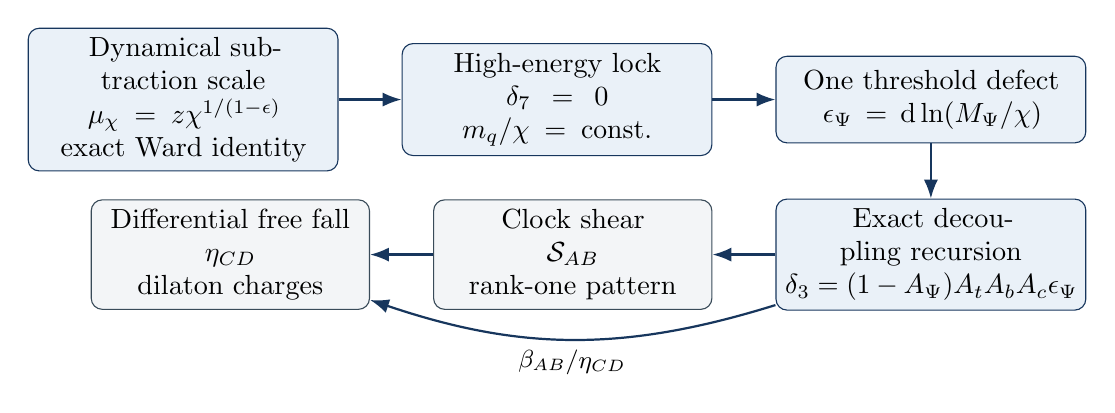
\begin{tikzpicture}[
node distance=7mm and 8mm,
box/.style={draw=navy,rounded corners,fill=lightblue,align=center,minimum height=11mm,text width=37mm},
small/.style={draw=slate,rounded corners,fill=lightgray,align=center,minimum height=10mm,text width=33mm},
arr/.style={-{Latex[length=2.4mm]},thick,draw=navy}
]
\node[box] (ward) {Dynamical subtraction scale\\$\mu_\chi=z\chi^{1/(1-\epsilon)}$\\exact Ward identity};
\node[box,right=of ward] (lock) {High-energy lock\\$\delta_7=0$\\$m_q/\chi=\mathrm{const.}$};
\node[box,right=of lock] (spurion) {One threshold defect\\$\epsilon_\Psi=\dd\ln(M_\Psi/\chi)$};
\node[box,below=of spurion] (qcd) {Exact decoupling recursion\\$\delta_3=(1-A_\Psi)A_tA_bA_c\epsilon_\Psi$};
\node[small,left=of qcd] (clock) {Clock shear\\$\mathcal S_{AB}$\\rank-one pattern};
\node[small,left=of clock] (ep) {Differential free fall\\$\eta_{CD}$\\dilaton charges};
\draw[arr] (ward)--(lock);
\draw[arr] (lock)--(spurion);
\draw[arr] (spurion)--(qcd);
\draw[arr] (qcd)--(clock);
\draw[arr] (clock)--(ep);
\draw[arr,bend left=18] (qcd) to node[below,sloped,font=\small] {$\beta_{AB}/\eta_{CD}$} (ep);
\end{tikzpicture}
\caption{The exact lock and its first controlled violation. The microscopic coefficient is needed to make the observables nonzero; it cancels in their same-source ratio.}
\end{figure}

\section{Novelty boundary and priority audit}

The literature search changes the priority claim substantially.

\subsection{Established ingredients}

The following components are established and must not be presented as new:

\begin{itemize}
  \item promoting the dimensional-regularization subtraction scale to a dilaton-dependent quantity;
  \item exact scale Ward identities with ordinary running in the spontaneously broken phase;
  \item the appearance of nonrenormalizable symmetry-restoring operators in manifestly scale-invariant regularization;
  \item all-orders QCD decoupling relations and heavy-mass low-energy theorems;
  \item the leading $2/27$ gluonic response of low-energy QCD to one heavy fundamental colour threshold;
  \item dilaton charges for test bodies and the relation between scalar fifth forces and variations of dimensionless constants;
  \item atomic and molecular clock sensitivity coefficients for $\alpha$ and $\mu$;
  \item suppression of a fifth force for an exactly universal scale mode.
\end{itemize}

These points are covered by Refs.~\cite{Tamarit2013,Ghilencea2016,HerreroValea2020,Chetyrkin1998,DamourDonoghue2010,Brzeminski2022,Elder2025,Ferreira2017}.

\subsection{Restricted candidate contribution}

The plausible original contribution is the following combined structure:

\begin{enumerate}
  \item define a QCD \emph{chronometric lock defect} $\delta_n=\dd\ln(\Lambda_n/\chi)$;
  \item derive the exact physical threshold recursion
  \[
  \delta_{n-1}=A_j\delta_n+(1-A_j)\epsilon_j;
  \]
  \item embed one finite renormalizable threshold-misalignment spurion in the otherwise universally locked scale theory;
  \item propagate it into the rank-one clock relation
  \[
  \mathcal S_{\rm Sr/Cs}=2\mathcal S_{\rm Sr/CaF};
  \]
  \item eliminate the unknown scalar amplitude to obtain the same-source line
  \[
  \beta_{AB}/\eta_{CD}
  =-(\Delta K_\mu-\Delta K_q)/\Delta Q'_{\widehat m}{}^{CD}.
  \]
\end{enumerate}

No exact indexed match for this restricted conjunction was found in the targeted search. That is not an absolute priority claim. The threshold recursion is mathematically simple once RGI variables are chosen, and the clock--EP relation may be implicit in existing dilaton phenomenology. A serious submission needs backward and forward citation chasing, INSPIRE and journal-database searches, and review by QCD decoupling and precision-clock specialists.

\section{What the result means for emergent time}

The new calculation does not make time arise from a QCD beta function. Its significance is more disciplined.

The exact common scale obeys
\[
\Lambda_{\QCD}=c_Q\chi,
\qquad
m_e=c_e\chi,
\qquad
\MP=c_P\chi.
\]
A universal rescaling of $\chi$ changes no local dimensionless clock ratio and corresponds to the common metric calibration developed in v0.3--v0.4. The first observable departure is not an arbitrary variation of ``time.'' It is the failure of one threshold to follow the common spectral scale:
\[
\epsilon_\Psi
=\dd\ln(M_\Psi/\chi)\neq0.
\]
Decoupling converts that failure into
\[
\delta_3
=\dd\ln(\Lambda_3/\chi)\neq0,
\]
and material clocks cease to agree on one universal spectral factor.

Thus the physical statement becomes
\[
\boxed{
\text{universal duration calibration}
=\text{rank-zero spectral response},
}
\]
while
\[
\boxed{
\text{chronometric shear}
=\text{RG-transmitted failure of universal scale locking}.
}
\]
The same shear produces composition-dependent scalar charge. Clock disagreement and equivalence-principle violation are therefore two views of one obstruction to metric universality.

\section{Final assessment and next calculations}

\statusbox{deepgreen}{\textbf{Result obtained.} The QCD step is no longer merely a local matching prescription. An explicit all-orders scale-invariant quantum functional gives the exact lock; an exact RGI decoupling theorem transports defects; and one ordinary renormalizable threshold produces the first nonzero clock--EP prediction.}

The status is:
\[
\boxed{
\begin{aligned}
\text{all-orders microscopic QCD lock}
&:\ \text{constructed as a Wilsonian EFT},\\
\text{finite UV completion}
&:\ \text{open},\\
\text{leading controlled violation}
&:\ \frac{2}{27}\varepsilon_\Psi\dd\theta,\\
\text{dimensionless clock test}
&:\ \mathcal S_{\rm Sr/Cs}=2\mathcal S_{\rm Sr/CaF},\\
\text{clock--EP test}
&:\ \beta_{AB}/\eta_{CD}
=-(\Delta K_\mu-\Delta K_q)/\Delta Q'_{\widehat m},\\
\text{natural observable long range}
&:\ \text{not yet solved}.
\end{aligned}}
\]

The next calculations should be performed in this order:

\begin{enumerate}
  \item Evaluate $A_\Psi,A_t,A_b,A_c$ with the highest available QCD beta functions and decoupling constants, including uncertainty from $\alpha_s$ and quark masses.
  \item Replace the leading $K_q=0$ benchmark by ab initio nuclear, hyperfine and molecular sensitivities, including the proton sigma terms.
  \item Construct a symmetry-protected ratio mode for which Eq.~\eqref{eq:radiativemass} is cancelled without introducing additional independent clock spurions.
  \item Fit the predicted rank-one vector jointly to clock-network and composition-dependent free-fall data rather than translating one bound into another.
  \item Test the exact scale-invariant QCD functional nonperturbatively by measuring whether dimensionless spectral ratios remain fixed when the background dilaton condensate is varied on a lattice.
\end{enumerate}

The third item is now the conceptual bottleneck. The QCD lock and its first defect are technically under control; making the defect both long-ranged and naturally large enough to observe is where new model building is required.

\appendix

\section{Symbolic and numerical verification}

The accompanying Python script performs the following independent checks:

\begin{enumerate}
  \item derives the scalar alignment Hessian and verifies
  \[
  \det H_{\rm total}
  =2\lambda_Sf^2r^2m_\chi^2;
  \]
  \item differentiates $M_\Psi/\chi$ and obtains
  \[
  \varepsilon_\Psi=\frac{y_Sr}{y_\chi+y_Sr};
  \]
  \item verifies the threshold-recursion algebra;
  \item computes
  \[
  A_\Psi=\frac{19}{21},\quad
  A_t=\frac{21}{23},\quad
  A_b=\frac{23}{25},\quad
  A_c=\frac{25}{27};
  \]
  \item verifies the telescoping coefficient $2/27$ and its generalization $4T(R)/27$;
  \item verifies Eqs.~\eqref{eq:srcaf}, \eqref{eq:srcs} and \eqref{eq:rankone};
  \item computes the Ti/Pt charges and Eqs.~\eqref{eq:150}--\eqref{eq:300};
  \item samples 50,000 positive lifted-completion scalar parameter points and finds no failed positive-definiteness test; the exact global-scale limit is obtained continuously at $m_\chi^2=0$ and is positive semidefinite.
\end{enumerate}

The machine-readable output records
\[
Q'_{\widehat m}({\rm Ti})=-0.01027656066,
\qquad
Q'_{\widehat m}({\rm Pt})=-0.00695167524,
\]
\[
\Delta Q'_{\widehat m}{}^{\rm Ti-Pt}
=-0.00332488542,
\]
and the coefficients $150.3811$ and $300.7622$.

\section{Conventions and caveats}

\begin{itemize}
  \item Natural units $\hbar=c=1$ are used except where a force range is converted to electronvolts.
  \item $\mu=m_p/m_e$, matching the clock-sensitivity convention of Ref.~\cite{Elder2025}.
  \item Ordered ratios matter. This note uses Sr/CaF, Sr/Cs and Ti minus Pt.
  \item The $Q'_{\widehat m}$ formula is a leading semi-empirical nuclear approximation, not isotope-resolved ab initio nuclear theory.
  \item ``All orders'' refers to the exact functional form and renormalized Wilsonian expansion. It does not mean every coefficient has been numerically calculated.
  \item The formal path-integral scale symmetry does not by itself prove reflection positivity, confinement or the existence of the desired vacuum. Conventional QCD evidence is inherited only in the broken, decoupling regime.
  \item The relation between anomalous redshift and Eotvos observables assumes one unscreened scalar and the same source. Screening, finite range and multiple fields alter it.
\end{itemize}

\begin{thebibliography}{99}

\bibitem{Tamarit2013}
C.~Tamarit,
``Running couplings with a vanishing scale anomaly,''
\emph{JHEP} \textbf{12} (2013) 098,
\href{https://arxiv.org/abs/1309.0913}{arXiv:1309.0913}.

\bibitem{Ghilencea2016}
D.~M.~Ghilencea,
``Manifestly scale-invariant regularization and quantum effective operators,''
\emph{Phys. Rev. D} \textbf{93} (2016) 105006,
\href{https://arxiv.org/abs/1508.00595}{arXiv:1508.00595}.

\bibitem{HerreroValea2020}
M.~Herrero-Valea,
``A Path (Integral) to Scale Invariance,''
\href{https://arxiv.org/abs/2007.04335}{arXiv:2007.04335} (2020).

\bibitem{Chetyrkin1998}
K.~G.~Chetyrkin, B.~A.~Kniehl and M.~Steinhauser,
``Decoupling Relations to $O(\alpha_s^3)$ and their Connection to Low-Energy Theorems,''
\emph{Nucl. Phys. B} \textbf{510} (1998) 61--87,
\href{https://arxiv.org/abs/hep-ph/9708255}{arXiv:hep-ph/9708255}.

\bibitem{DamourDonoghue2010}
T.~Damour and J.~F.~Donoghue,
``Equivalence Principle Violations and Couplings of a Light Dilaton,''
\emph{Phys. Rev. D} \textbf{82} (2010) 084033,
\href{https://arxiv.org/abs/1007.2792}{arXiv:1007.2792}.

\bibitem{Brzeminski2022}
D.~Brzeminski, Z.~Chacko, A.~Dev, I.~Flood and A.~Hook,
``Searching for a Fifth Force with Atomic and Nuclear Clocks,''
\emph{Phys. Rev. D} \textbf{106} (2022) 095031,
\href{https://arxiv.org/abs/2207.14310}{arXiv:2207.14310}.

\bibitem{MICROSCOPE2022}
P.~Touboul et al.,
``MICROSCOPE Mission: Final Results of the Test of the Equivalence Principle,''
\emph{Phys. Rev. Lett.} \textbf{129} (2022) 121102,
\href{https://arxiv.org/abs/2209.15487}{arXiv:2209.15487}.

\bibitem{Elder2025}
B.~Elder, G.~Mentasti, E.~Pasatembou et al.,
``Prospects for detecting new dark physics with the next generation of atomic clocks,''
\href{https://arxiv.org/abs/2504.07179}{arXiv:2504.07179} (2025).

\bibitem{Ferreira2017}
P.~G.~Ferreira, C.~T.~Hill and G.~G.~Ross,
``No fifth force in a scale invariant universe,''
\emph{Phys. Rev. D} \textbf{95} (2017) 064038,
\href{https://arxiv.org/abs/1612.03157}{arXiv:1612.03157}.

\end{thebibliography}

\end{document}
